\documentclass[12pt]{extarticle}

% polski font
\usepackage[T1]{fontenc}
\usepackage[polish]{babel}
\usepackage[utf8]{inputenc}
\selectlanguage{polish}

% wykresy
\usepackage{graphicx}

% arial
\renewcommand{\rmdefault}{phv}
\renewcommand{\sfdefault}{phv}

% kropki po numerach nagłówków
\usepackage{titlesec}
\titlelabel{\thetitle.\quad}

% kropki w labelkach rysunków itp.
\usepackage[labelsep = period]{caption}

% interlinia
\linespread{1.25}

% wyłączenie łamania słów i justowanie
\usepackage[none]{hyphenat}
\sloppy

% wcięcie na pierwszych liniach rozdziałów
\usepackage{indentfirst}

% klikalne linki
\usepackage[colorlinks, linkcolor=blue]{hyperref}

% dane dokumentu
\title{Praca inżynierska}
\author{Amadeusz Hercog}
\date{21 listopada 2018}

\begin{document}
	\pagenumbering{gobble}
	\maketitle
	
	\newpage
	\pagenumbering{arabic}
	\section{Opis symulatora}	
	Symulator użyty w projekcie jest programem napisanym w języku C++ autorstwa Roberta Lubaś oraz Wojciecha Myśliwiec. Służy on do modelowania ruchu agentów (ludzi) podczas ewakuacji w danej przestrzeni. Symulowana przestrzeń jest dwuwymiarowa, z możliwością dodania wielu poziomów odpowiadających kolejnym piętrom budynku. Główne okno programu jest widoczne na \hyperref[fig: glowne_okno_symulatora]{rysunku 1}.

	\begin{figure}[h]
 		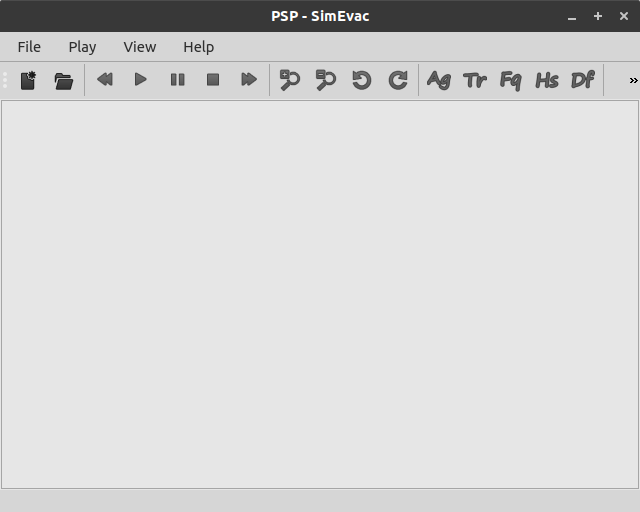
\includegraphics[width = \linewidth]{rysunki/symulator.png}
		\caption{Główne okno symulatora.}
		\label{fig: glowne_okno_symulatora}
	\end{figure}
	
		\subsection{Sposób użycia}
		Do przeprowadzenia symulacji potrzebne są następujące rzeczy:
		\begin{itemize}
		\item plik \textit{.xml} zawierający parametry wejściowe symulacji,
		\item pliki \textit{.jpg} i \textit{.bmp} zwierające przestrzeń użytą do symulacji.
		\end{itemize}
	
		W oknie głównym programu należy wybrać opcje otwarcia pliku \textit{.xml} po czym od razu zaczyna się symulacja w czasie rzeczywistym. Po symulacji, we wskazanym w pliku z parametrami folderze zostaną wygenerowane pliki \textit{.csv} z danymi wyjściowymi symulacji.
		
		\subsection{Dane wejściowe i wyjściowe}
		Dane, na których miałem możliwość przeprowadzenia badań znajdowały się w:
		\begin{itemize}
		\item dane wejściowe - plik \textit{.xml},
		\item dane wyjściowe - pliki \textit{.csv}.
		\end{itemize}
		
		Danymi wejściowymi, które wybrałem - na podstawie łatwości modyfikacji - do dalszej analizy były:
		
		\begin{itemize}
		\item \textbf{Panic spread factor} - współczynnik, który decyduje jak duzy wpływ ma \textbf{tryb paniki} (tryb, w którym agenci zwracają mniejszą uwagę na otoczenie oraz charakteryzują się bardziej chaotycznym ruchem) na agentów.
		\item \textbf{Panic cancel zone} - współczynnik określający odległość od wyjść, w obrębie jakiej agenci mają szansę na deaktywację trybu paniki.
		\item \textbf{Cancel panic chance}- podczas testów na anulowanie trybu paniki określa procent szans na powodzenie.
		\item \textbf{Choosing evacuation path mode} - tryb wyboru drogi ewakuacyjnej przez agentów. Dostępne są 4 tryby:
			\begin{itemize}
			\item odległości,
			\item gęstości przy wyjściu,
			\item odległości oraz gęstości przy wyjściu,
			\item odległości, gęstości przy wyjściu oraz popularności wyboru wyjścia.
			\end{itemize}
		\item \textbf{Number of pederastians} - liczba agentów biorąca udział w symulacji.
		\item \textbf{Chaos level} - szansa na aktywację trybu paniki u agentów.
		\item \textbf{Density factor} - określa wpływ współczynnika gęstości wokół agenta na funkcję kary.
		\item \textbf{Frequency factor} - określa wpływ częstości wyboru danego pola na funkcję kary.
		\item \textbf{Panic factor} - zwiększa część współczynników biorących udział w obliczaniu funkcji kary. 
		\item \textbf{Distance factor} - wpływa na wybór agentów ruchu po skosie lub na wprost.
		\item \textbf{Randomness factor} - czynnik losowości dla wartości kary.
		\item \textbf{Pre-movement time mean value} oraz \textbf{Pre-movement time standard deviation} - średnia i odchylenie czasu \textit{Pre-movement}, który ma wpływ na częstotliwość wykonywania testu na zmianę obranego wyjścia przez agentów.
		\item \textbf{Speed distribution mean value} oraz \textbf{Speed distribution standard deviation} - średnia i odchylenie prędkości agentów.
		\end{itemize}
		
		Dane wyjściowe wybrane wybrane do analizy przeze mnie były następujące:
		
		\begin{itemize}
		\item czas ewakuacji osatatniego agenta (odpowiadający czasowi ewakuacji wszystkich agentów),
		\item błąd średniokwadratowy średnich prędkości wszystkich agentów w stosunku do średniej prędkości najszybszego agenta.
		\end{itemize}
\end{document}
